\documentclass[12pt,twocolumn,letterpaper]{article}

\usepackage{cvpr}
\usepackage{times}
\usepackage{epsfig}
\usepackage{graphicx}
\usepackage{amsmath}
\usepackage{amssymb}
\usepackage{algorithm}
\usepackage{algpseudocode}
\usepackage{float}

% Include other packages here, before hyperref.

% If you comment hyperref and then uncomment it, you should delete
% egpaper.aux before re-running latex.  (Or just hit 'q' on the first latex
% run, let it finish, and you should be clear).
\usepackage[breaklinks=true,bookmarks=false]{hyperref}

\cvprfinalcopy % *** Uncomment this line for the final submission

\def\cvprPaperID{****} % *** Enter the CVPR Paper ID here
\def\httilde{\mbox{\tt\raisebox{-.5ex}{\symbol{126}}}}

% Pages are numbered in submission mode, and unnumbered in camera-ready
%\ifcvprfinal\pagestyle{empty}\fi
\setcounter{page}{1}
\begin{document}

%%%%%%%%% TITLE
\title{Investigation of Impact of Auxiliary Tasks and Auxiliary Tasks Weight Autoadjustment}

\author{Benjamin Liu\\
UC Berkeley\\
{\tt\small benjamin.liu@berkeley.edu}
\and
Zhaoxin Gu\\
UC Berkeley\\
{\tt\small zgu14@berkeley.edu}
}

\maketitle
%\thispagestyle{empty}

%%%%%%%%% ABSTRACT
\begin{abstract}
	People’s interest in AI has grown at an incredible speed during the recent years. Reinforcement Learning is surely has it’s application. As the application of Reinforcement Learning expands, the amount of data grows, and the complexity of the algorithms raise,to improve the time that required to train a decent Reinforcement Learning agent and to improve the performance of the agent have been areas that a lot of researches has focused on. One way to improve the performance of the agent and the amount of time required to train such agent is by using Auxiliary Tasks. The idea of using Auxiliary task is to give Auxiliary goals to speed up the training process and boost the final performance. Some researches focusing on auxiliary tasks have been done in the past and laid the foundation of our project. 

Our project focuses on investigating the effect of different numbers of auxiliary tasks has in the performance of the RL agent and developing a novel method of automatically adjust the weights associated with different auxiliary tasks. To our knowledge, even though people have looked at various auxiliary tasks, no one has looked into how different number of auxiliary tasks affect the performance if the agent, nor do people has developed an automatic weight adjustment algorithm. 

In our project, we used A3C\textsuperscript{[3][4]} as our baseline method to speedup the training process. The auxiliary tasks (Value Replay, Pixel Control, and Reward Prediction) we investigated are based on Reinforcement Learning with Unsupervised Auxiliary Tasks\textsuperscript{[2]}. Based on our results from the experiments, we concluded that adding more similar tasks will not have significant effect on the agent. 

We also implemented an algorithm that automatically adjust the weights of different tasks. Based on the result, our algorithm was able to achieve a better convergence rate and a comparable results after adequate amount of training.

As a team, both member contributed to the project. Benjamin Liu primarily focused on literature reviews, running experiments, modifying existing code in order to adjust the weight, debugging the automated weight adjustment algorithm, and analyzing the results from the experiments. Whereas Zhaoxin Gu came up with plans from the project, focused on running experiments, implementing the automated weight adjustment algorithm, debugging the code and analyzing the results.

\end{abstract}

%%%%%%%%% BODY TEXT
\section{Background and Introduction}

%-------------------------------------------------------------------------
\subsection{Reinforcement Learning}

In the standard reinforcement learning setting, at each discrete time step t, an agent observes state st S and rewards rt and it, based on certain policy pi, chooses action at from action space A which will affect states and rewards for the future. The value function is $V^{\pi}(s) = \mathbb{E}_\pi[R_{t}|s_t = s]$. The Q function is $Q^{\pi}(s, a) = \mathbb{E}_\pi[R_t|s_t = s, a_t = a]$ . The advantage function is $A^{\pi}(s, a) = Q^{\pi}(s, a) - V^{\pi}(s)$. The goal of reinforcement learning is, by learning an optimal decision policy $\pi(a'|s, a)$, maximizing the total discounted trajectory rewards $R_t = \sum_{k=0}^{\infty}\gamma^k r_{t+k}$ at time step t.

The model-free approach to reinforcement learning includes value-based algorithms and policy-based algorithms. Value-based reinforcement learning algorithms, such as Deep Q Network\textsuperscript{[3]} (Mnih et al., 2015) and Deep Deterministic Policy Gradient\textsuperscript{[11]} (Lillicrap et al, 2015), approximate Q function $Q_\theta^\pi(s, a)$ by parameters $\theta$ and then update parameters by applying gradient ascent. Policy-based reinforcement learning algorithms, such as Trust Region Policy Optimization\textsuperscript{[12]} (Schulman et al., 2015) and Proximal Policy Optimization\textsuperscript{[13]} (Schulman et al, 2017), model a policy $\pi_\theta(a'|s, a)$, parametrized by theta. Taking gradients with respect to $\theta$ for $L_\pi = \mathbb{E}_{s\sim\pi}[R_t]$, the agent use stochastic gradient ascent to maximize the expected trajectory rewards.

%-------------------------------------------------------------------------
\subsection{Atari 2600 Games in Arcade Learning Environment}

%-------------------------------------------insert a big figure------------------------
\begin{figure*}
\begin{center}
\fbox{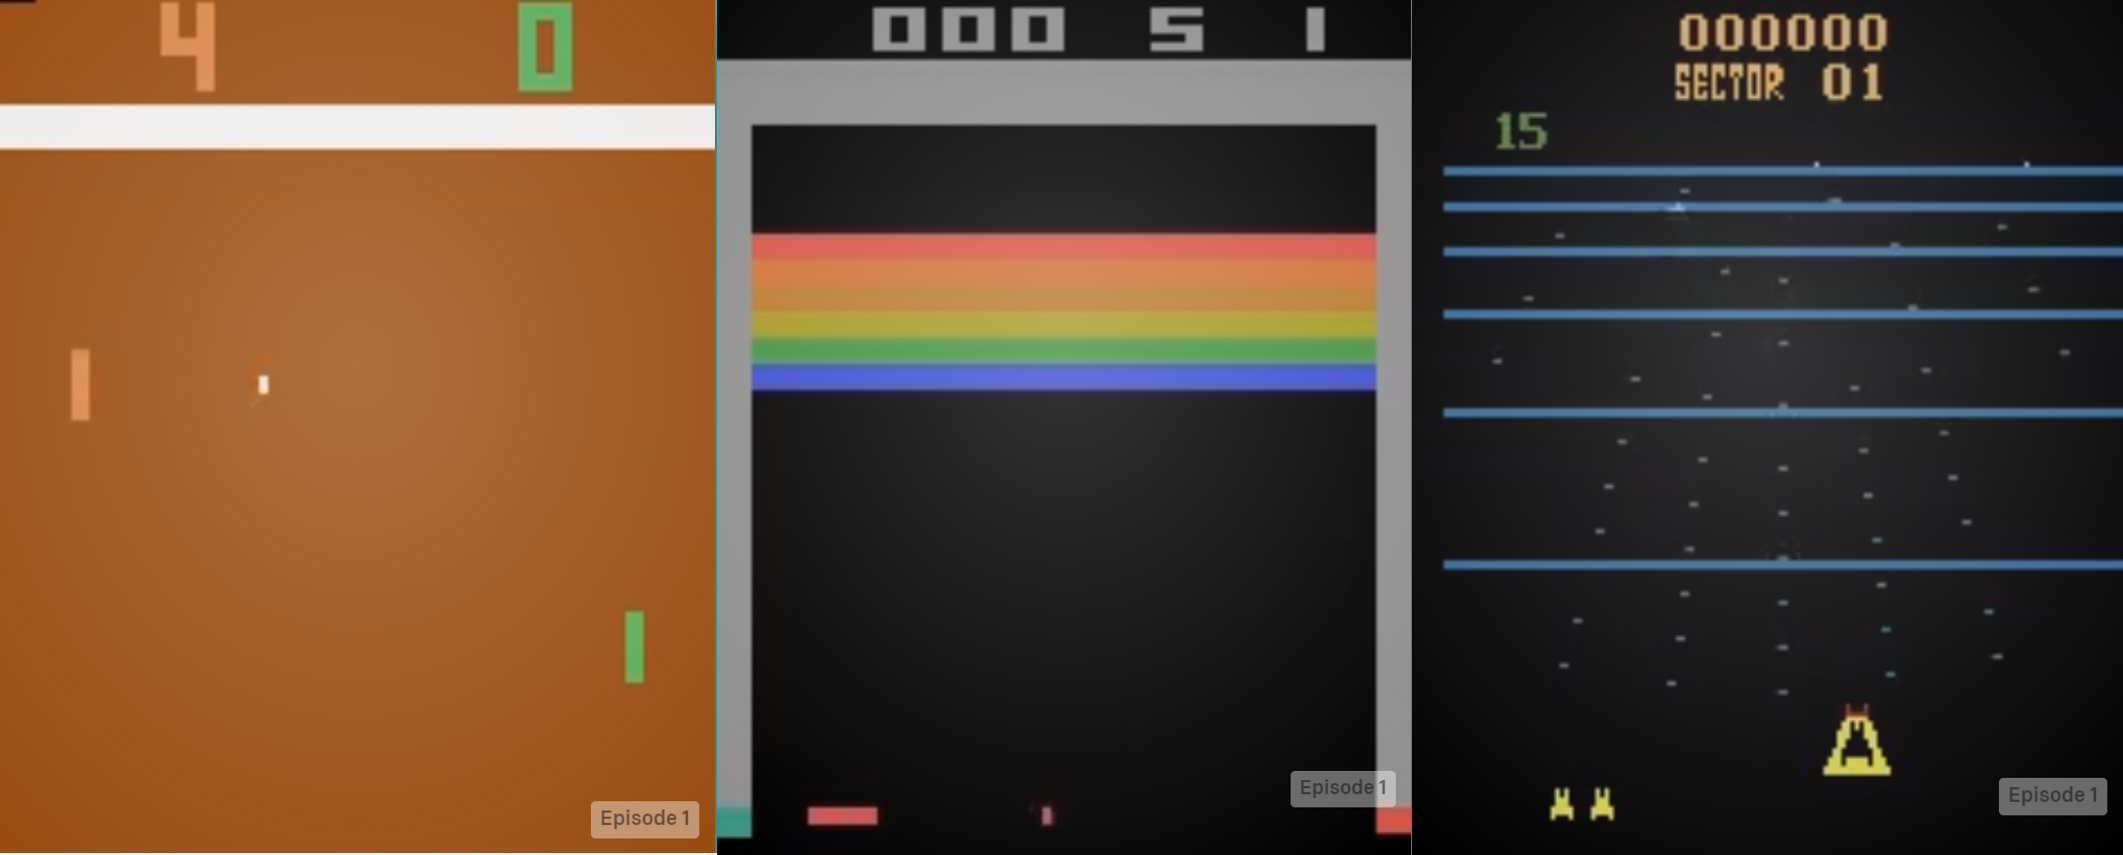
\includegraphics[width=15cm, height=4.5cm]{atari.png}}
\end{center}
   \caption{Game Pong, Breakout and BeamRider.}
\label{fig:short}
\end{figure*}

The Arcade Learning Environment\textsuperscript{[5]} (Bellemare et al., 2012) provides simulator and evaluation platform for playing Atari 2600 games. ALE provides multiple different Atari simulation environments. For example, for Pong game, different environments include \textit{Deterministic, NoFrameskip, RAM, RAMDeterministic and RAMNoFrameSkip}\textsuperscript{[10]} can be experimented with. In the past five years, ALE received great attention from the reinforcement learning research community and many classical reinforcement learning algorithm have been experimented in ALE by previous researchers. We can do sanity check with our implemented model by comparing with similar architecture tested in ALE. In the experiment, we also use the classical reinforcement learning algorithm A3C's performance as the comparison benchmark. 

At the same time, Atari 2600 Games are excellent domain for evaluating reinforcement learning agents. Firstly, the state space $S$, action space $A$, and especially, rewards $r$ are all well-defined. In addition, the game itself also embeds complex interactive dynamics in which state-of-the-art reinforcement learning is more likely to outperform other learning methods. Lastly, a human expert, say an experienced gamer, can do reasonably good in some games, which brings us more insights about human decision making in a Markov Process and hopefully helps the computer agents to achieve rewards closed to or exceed human experts.


\section{Related Works}
%-------------------------------------------------------------------------
\subsection{A3C Algorithm}
The Actor-Critic algorithm can be treated as a natural extension of policy gradient method. The Actor collects experience ${(s_t, a_t, r_t)}$ based on decision policy $\pi(a'|s, a)$ and optimize its policy with respect to total discounted rewards $R_t$ at each time step t (aka doing policy gradient updates). The Critic is function approximation for value function $\hat{V}_\phi^\pi(s)$ and, at each time step t, $\hat{V}_\phi^\pi(s)$ is fitted to the sum of discounted rewards from sampled experience. 

% ----------------------------------------insert a small figure----------------------------
\begin{figure}[t]
\begin{center}
\fbox{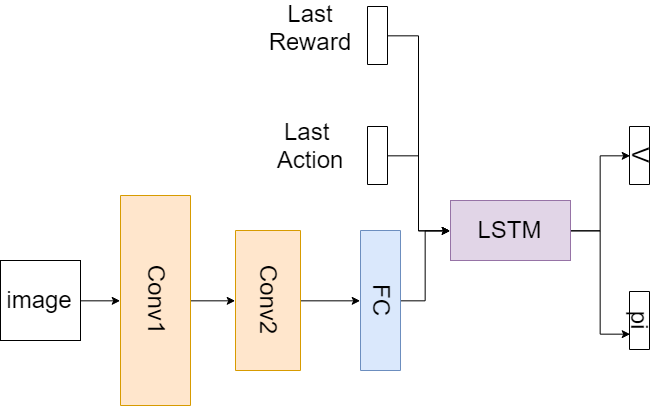
\includegraphics[width=8cm, height=4cm]{A3C.png}}
\end{center}
   \caption{A3C Network Architecture}
\label{fig:long}
\label{fig:onecol}
\end{figure}

One recent advance in Actor-Critic style algorithm is \textit{A3C}, the \textit{Asynchronous Advantage Actor-Critic}\textsuperscript{[3]} (Mnih et al, 2016). The novelty of A3C is that, just like GORILA\textsuperscript{[4]} (Nair et al, 2015), it allows asynchronous learning by using multiple workers and one parameter server, which makes the parallelized learning accelerated and the training data decorrelated. In a A3C framework, instead of, like in a conventional actor-critic way, executing one worker to interact with environment at a time , several workers are collecting experience ${(s_t, a_t, r_t)}$ in its own environment and compute the gradients in parallel. For each worker, there are two neural networks, one for policy $\pi_\theta(s, a)$ and the other for value function $V_\theta(s)$. The parameter server, a global neural network take in the gradients periodically, perform parameter update, and synchronize the network parameter with all asynchronous workers' network. Since advantage function has the benefit of variance reduction, the global network parameter gradient computation is based on advantage function $A^\pi(s, a)$. 
$$L_{A3C} = L_\pi + \mathbb{E}_{s\sim\pi}[A^\pi(s, a)^2] - \mathbb{E}_{s\sim\pi}[\beta H(\pi)] $$

In order to prevent convergence to local optima, an entropy penalty term $\beta H(\pi)$ is subtracted in the gradient update. For the optimizer, an RMSProp optimizer is used (described below).
$$ g_t = \nabla_\theta L_{A3C, t} $$
$$ \nu_t = \alpha \nu_t + (1-\alpha) g_t^2 $$
$$ \Delta \theta_t = - \frac{\eta}{\sqrt[]{\nu_t + \epsilon}} g_t$$
$$ \theta_{t+1} = \theta_t + \Delta \theta_t $$




%-------------------------------------------------------------------------
\subsection{UNREAL Auxiliary Tasks}
The \textit{UNREAL} agent stands for \textit{UNsupervised REinforcement and Auxiliary Learning} agent\textsuperscript{[2]} (Jaderberg et al, 2016). Basically, unsupervised auxiliary tasks, such as pixel control, feature control, value replay and reward prediction, are added on top of the A3C agent. The losses defined for each auxiliary tasks will be combined using weights $\lambda$, which produce a single loss function $L_{UNREAL}$ for the UNREAL agent. Then, the optimizer perform gradient steps on parameters $\theta$ with respect to combined loss function $L_{UNREAL}$. 

$$ L_{UNREAL} = L_{A3C} + \lambda_{VR} L_{VR} + \lambda_{PC} L_{PC} + \lambda_{RP} L_{RP} $$
where $\lambda_{VR}, \lambda_{PC}, \lambda_{RP}$ are weights on the individual loss components.

\subsubsection{Pixel Control}
Pixel control is an auxiliary control task. The intuition is that large changes in image correspond to important events in training domain. For the pixel control task, a policy that controls the input image pixel changes is trained via loss function.
$$ L_{PC} = (Q_{PC}(s_t, a_t) - $$
$$ \sum_{i = 0}^{k-1}[\gamma^i r_{t+i} + \gamma^k \max_{a}Q_{PC}(s_{t+k}, a)])^2$$ 

% ----------------------------------------insert a small figure----------------------------
\begin{figure}[H]
\begin{center}
\fbox{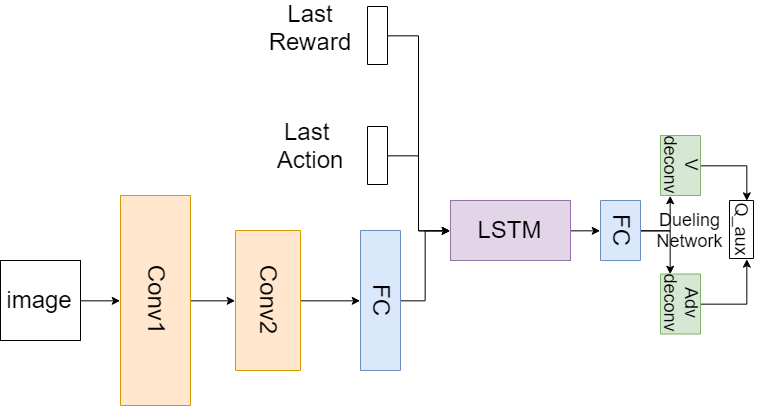
\includegraphics[width=8cm, height=4cm]{PC.png}}
\end{center}
   \caption{Pixel Control Network Diagram}
\label{fig:long}
\label{fig:onecol}
\end{figure}

\subsubsection{Value Replay}
Value replay is an auxiliary experience replay task. In a DQN framework[3] (Mnih et al., 2016), implementing experience replay buffer is beneficial for improving data efficiency and break the data correlation. The idea is similar for the task value replay which resample recent trajectories and extra regression is performed to better approximate value function $V^\pi(s)$.
% ----------------------------------------insert a small figure----------------------------
\begin{figure}[H]
\begin{center}
\fbox{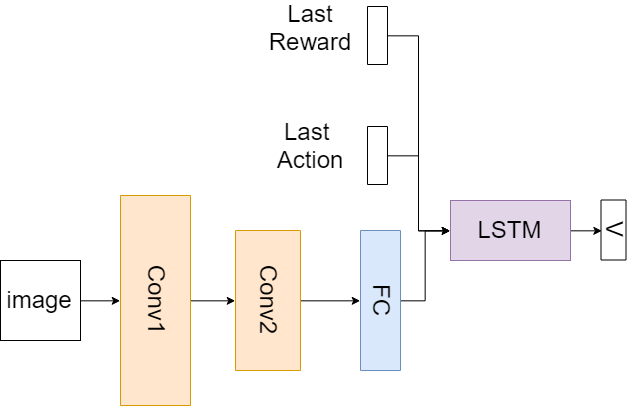
\includegraphics[width=8cm, height=4cm]{VR.png}}
\end{center}
   \caption{Value Replay Network Diagram}
\label{fig:long}
\label{fig:onecol}
\end{figure}

\subsubsection{Reward Prediction}
Reward prediction is an auxiliary reward task. The intuition is that learning reward prediction helps agent to identify state observations that lead to desirable outcomes. For the reward prediction task, the past three state observations $s_t$, $s_{t-1}$, $s_{t-2}$ are input to a network to predict whether next reward $r_{t+1}$ is positive, negative, or zero. 
% ----------------------------------------insert a small figure----------------------------
\begin{figure}[H]
\begin{center}
\fbox{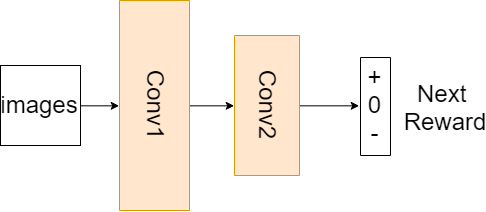
\includegraphics[width=8cm, height=4cm]{RP.png}}
\end{center}
   \caption{Reward Prediction Network Diagram}
\label{fig:long}
\label{fig:onecol}
\end{figure}


\subsubsection{Automated Weight Adjustment}
While conducting the experiments on the effects of various number of tasks on the RL agent, we didn’t tune the weights of different tasks. This motivated us to figure out a way to change the weight automatically. Inspired by Evolved Policy Gradient[1], we implemented an algorithm to adjust the weight automatically. The main idea is that the automatic weight adjustment algorithm should increase the weight associated to the task that can aid the baseline network to reach the highest overall rewards and decrease the weight of the task that achieves the lowest overall reward. 

In order to determine which task assists the baseline method the best, we first need to compare the overall reward that each tasks can reach. Our algorithm starts by training each task with the baseline method individually and record the total reward of each task after a short amount of training steps for comparison. To be fair, all tasks are trained from the same starting point and same baseline network and from there, each model are allowed to be trained freely. After all the rewards are collected, the algorithm first adjusts the weights of the tasks based on the rewards and then trains the baseline network with all tasks with new weights. The initial baseline network being used is the one before each individual tasks are trained. And after a certain amount of training step, the algorithm evaluates the tasks again and updates the weight to start a new iteration of training. 

Below is a pseudo code of the overall algorithm:
\begin{algorithm}[H]
\caption{Overall Algorithm}\label{euclid}
\begin{algorithmic}[1]
\Procedure{}{}
    
	\For{\textit{ K training iterations}}
		\For{\textit{each task}}
			\State \textit{Reset the environment}
			\State \textit{Load baseline network}
			\State \textit{Train the baseline and task for N steps and record total reward};
		\EndFor{}
	\State \textit{Update the weight of each task base on the reward}
	\State \textit{Load the baseline network and environment}
	\State \textit{Train the baseline network with all tasks for M steps}
	\State \textit{Store the baseline network and the environment};
	\EndFor{}

\EndProcedure
\end{algorithmic}
\end{algorithm}

The total amount of training step that the final baseline network takes is K x M steps.


\section{Experiments}
%-------------------------------------------------------------------------
\subsection{Impact of Number of Auxiliary Tasks}
First, we experiment playing Atari games with different number of auxiliary tasks. For example, for Breakout game, we experiment with only one auxiliary task, two auxiliary tasks and three auxiliary tasks, while keeping all the other hyperparameters, including the weights lambda the same.

The implementation details for basic A3C are as follows:
\begin{quote}

	The input is 84 x 84 images. The input will be first passed to a convolution layer with 16 8 x 8 filters and stride is 4. The next convolution layer 32 4 x 4 filters and stride is 4. The third layer is a fully connected layer with 256-units. ReLU activation function is used. All agents use LSTM with forget gates with 256 cells to process the CNN-encoded observation, previous action and current reward. 

\end{quote}

The implementation details for Pixel Control, Reward Prediction and Value Replay are as follows:

\begin{quote}

	For pixel control, one network policy is trained to control central 80 x 80 window of image. In fact, we look at a 20 x 20 grid of non-overlapping 4 x 4 cells. The reward for each 4 x 4 cells is defined as average absolute difference from previous frame. The LSTM produce outputs and the outputs are mapped into a 32 x 7 x 7 spatial feature map with a linear layer followed by ReLU nonlinearity. The next deconv layers with 1 and $N_{action}$ 4 x 4 filters and stride 2 map 32 x 7 x 7 into a value tensor and a advantage tensor. Using dueling parametrization, the spatial map is decoded into Q-function $N_{action}$ x 20 x 20 $Q^{aux}$.

For reward prediction, three observations $s_{t-2}$, $s_{t-1}$, $s_t$ are fed through three instance of agent’s CNN. The outputs from CNN are concatenated to feed through a 128-units fully connected layer. The ReLU non-linearity is applied. The final layer use softmax to predict the next reward $r_{t+1}$ to be positive, negative or zero. The value function replay is performed on a sequence of length 20.

\end{quote}

\subsection{Automated Weight Adjustment Experiment Setup}
Due to limiting time and the long training time for agents with inputs based on images from Atari games, we only conducted one experiment for the algorithm. We tested our automated weight adjustment algorithm using Atari game Pong since base on our experiments with different number of auxiliary tasks, we noticed that training on Pong is guaranteed to converge under 10M steps.

We set our total training step for our baseline network to be 8M step. Again, base on the results from prior experiments, 8M step is sufficient for the agent to converge. The frequency for updating the weight is set to every 0.1M steps. This means the weights will be updated 80 times throughout the training session. The number of steps for training each individual task before the evaluation is set to 10K steps. In this case, approximately 10\% of the time is evaluating the performance of each individual task. For the weight of each auxiliary task, the weights were initialized as follow:

\begin{table}[H]
\centering
\begin{tabular}{|l|l|}
\hline
Pixel Control:     & 0.001 \\ \hline
Value Replay:      & 1     \\ \hline
Reward Prediction: & 1     \\ \hline
\end{tabular}
\end{table}

The initial weights were selected based on the values used in the original paper\textsuperscript{[1]}, and we believe these would serve as good starting points for our algorithm.
The update rate for the weights were set to +/- 15\%. This means that after the evaluation of the performance of each task, the weight of the best performing one will be increased by 15\% while the least performing one will be decreased by 15\% and the one in the middle is being kept the same. 


\section{Results}
%-------------------------------------------------------------------------
\subsection{Effect of Number of Auxiliary Tasks}
The first phrase of our experiment is evaluating the effect of number of auxiliary tasks on the reinforcement learning agent performance in moderate complex settings like Atari. As mentioned above, our baseline performance is the vanilla A3C algorithm and we compare the convergence speed and maximum rewards of different number of auxiliary tasks with A3C results. 

We experiment our implemented algorithm (described in section 3.1) with Atari games, such as \textit{Pong, Breakout, BeamRider}. The learning curve of reinforcement learning agent under different auxiliary tasks settings for each game is presented in Figure 6. 

% ----------------------------------------insert a small figure----------------------------
\begin{figure}[H]
\begin{center}
\fbox{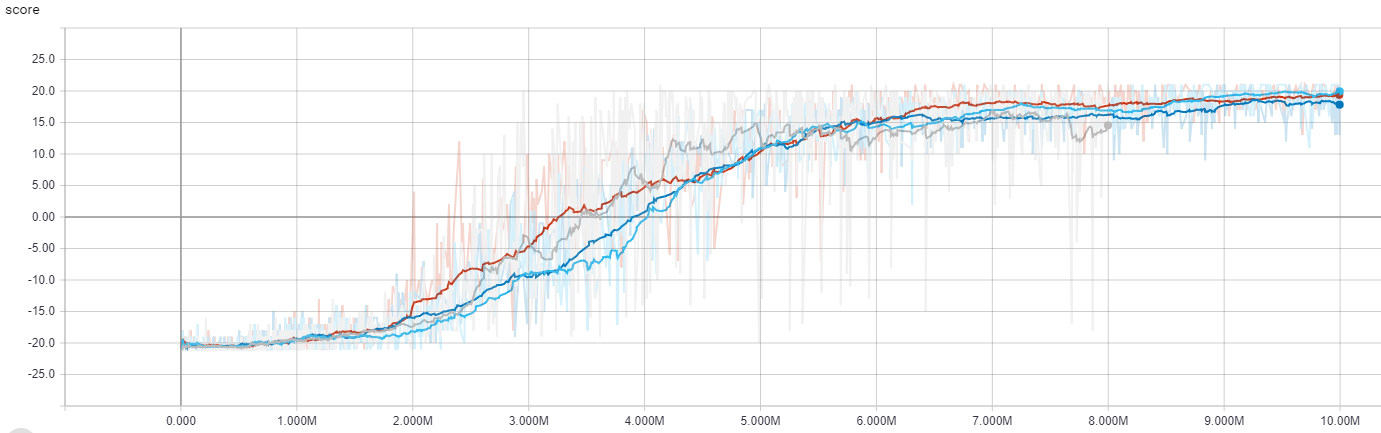
\includegraphics[width=8cm, height=4.8cm]{pong.png}}
\end{center}
\begin{center}
\fbox{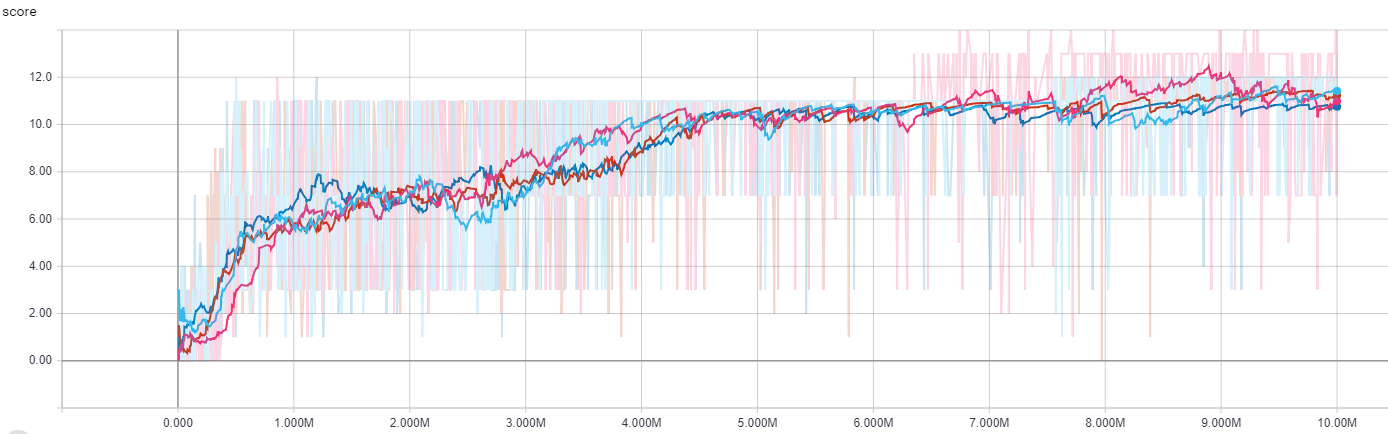
\includegraphics[width=8cm, height=4.8cm]{breakout.png}}
\end{center}
\begin{center}
\fbox{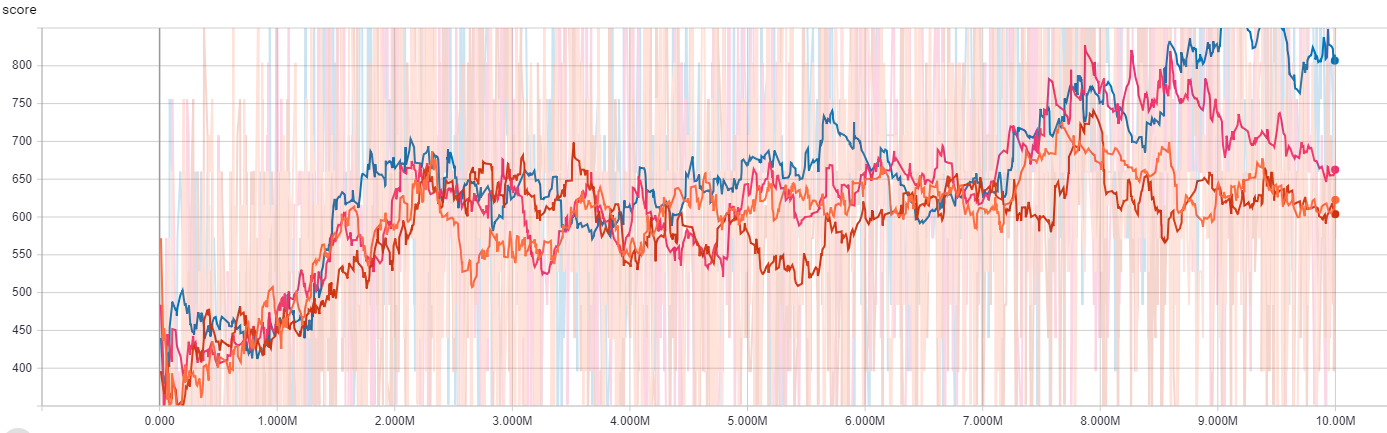
\includegraphics[width=8cm, height=4.8cm]{beamrider.png}}
\end{center}
	\caption{Top to bottom, results from different setups for training on Pong, Breakout and Beamrider. Pong: Dark blue is A3C; Red is 1 task; Light blue is 2 tasks; Gray is 3 tasks. Breakout: Dark blue is A3C; Purple is 1 task; Light blue is 2 tasks; Brown is all 3 tasks. Beamrider: Orange is A3C; Purple is 1 task; Brown is 2 tasks; Dark blue is all 3 tasks.}
\label{fig:long}
\label{fig:onecol}
\end{figure}


We found that 1) Adding one single auxiliary task can increase speed of convergence and final maximum rewards. 2) However, adding more similar auxiliary tasks won’t lead to significant improvement. We conclude that adding more similar auxiliary tasks is irrelevant with algorithm performance. Our team's hypothesis is that only devising innately different auxiliary tasks can be helpful, but it usually requires human intuitions.

%-------------------------------------------------------------------------
\subsection{Automatic Weight Adjustment Experiment Result}
The result of the experiment for the automatic weight adjustment algorithm with 8M total training steps, updating the weight every 0.1M steps, 10K steps training for each task before evaluation and a +/-15\% percent weight adjustment is shown in figure 7. From figure 7, we notice that our algorithm was able to achieve a comparable final result of an average reward of 17 and the algorithm converges around 4.4M steps which is faster than other experiments setups. We also noticed that there were some randomness so the results from experiments with same setups produced slightly different results.

% ----------------------------------------insert a small figure----------------------------
\begin{figure}[H]
\begin{center}
\fbox{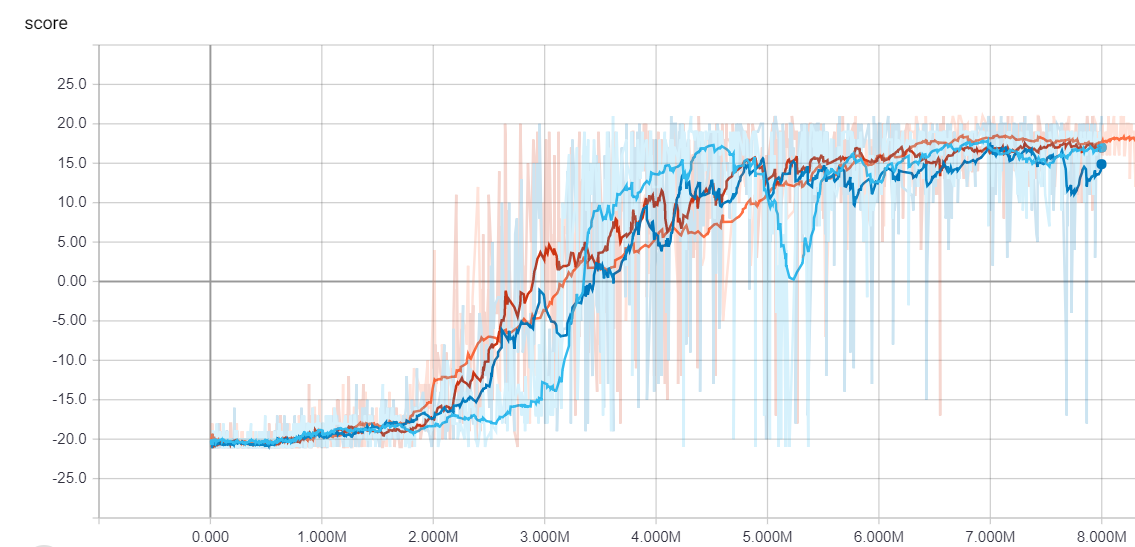
\includegraphics[width=8cm, height=5cm]{auto.png}}
\end{center}
   \caption{Results from different setups for training on Pong. 
Light blue: Automated weight adjustment;
Orange: A3C only; Dark blue: three tasks with fixed weights
Red:A3C with two auxiliary tasks}
\label{fig:long}
\label{fig:onecol}
\end{figure}

\section{Conclusion}
% choose weightys automatically?
The first part of our experiment studied the effect of number of auxiliary tasks on the performance of A3C algorithm. The experiment results convinced us that, while having one auxiliary task is helpful, adding more similar auxiliary tasks won't improve the the convergence speed nor maximum reward. Hence, instead of attempting to add more tasks to improve the original UNREAL agent, we choose to further investigate a method to choose the weights of each tasks' cost automatically via meta-learning. 
 
Based on our result from the experiment, our algorithm achieved a good performance and accomplished our initial goal of adjusting the weights to speed up convergence and boost performance. Our algorithm was able to achieve a faster convergence than any other experiments with fixed weights. The algorithm can be very helpful for choosing the weight of each task and can save a great amount of time when comparing to choosing a set of fixed weights for the tasks manually. With a higher weight update rate and a balanced percentage of steps for training each task individually before evaluation, we believe the algorithm can achieve a better performance by generating the optimum weights faster and more accurately.


\section{Future Work}
Due to time constraints, we only conducted experiment on certain environments with limited training steps. For example, training the agent on Atari game Breakout with 10M wasn’t enough for the agent to converge. And our experiments mainly ran on Pong due to the fast convergence of the agent in the given environment. In order to more accurately evaluated the effect of various number of tasks, more experiments with a more diverse environment and more training steps can be conducted.

More experiments with different environment, training steps, training intervals, task evaluation frequencies and different weight changing rate should also be done so that the effectiveness of the automated weight adjustment algorithm can be more accurately evaluated.

Another direction that can be examined is to come up with a target for the weights so that a gradient can be computed in order to update the weight more accurately.


\section{Reference}
[1] Houthooft, et, al. “Evolved policy gradient” arXiv preprint arXiv: 1802.04821 (2018)

[2] Jaderberg, Mnih, et al. “Reinforcement Learning with Unsupervised Auxiliary Tasks” arXiv preprint arXiv:1611.05397 (2016)

[3]  Mnih, et al. “Asynchronous Methods for Deep Reinforcement Learning” arXiv preprint arXiv:1602.01783 (2016)

[4] Nair, et al. “Massively Parallel Methods for Deep Reinforcement Learning” arXiv preprint arXiv:1507.04296 (2015)

[5] Bellemare, et al. “The Arcade Learning Environment: An Evaluation Platform for General Agents” arXiv preprint arXiv:1207.4708 (2012)

[6] Machado, et al. “Revisiting the Arcade Learning Environment: Evaluation Protocols and Open Problems for General Agents” arXiv preprint arXiv:1709.06009 (2017)

[7] Mnih, et al. “Playing Atari with Deep Reinforcement Learning” arXiv preprint arXiv:1312.5602 (2013)

[8] Johnson. “Surprise Pursuit Auxiliary Task for Deepmind Lab Maze” http://cs231n.stanford.edu/reports.html (2017)

[9] https://github.com/miyosuda/unreal 

[10]https://qiita.com/keisuke-nakata/items/141fc53f419b102d942c 

[11] Lillicrap, et al. “Continuous Control with Deep Reinforcement Learning” arXiv preprint arXiv:1509.02971 (2015)

[12] Schulman, et al. “Trust Region Policy Optimization” arXiv preprint arXiv:1502.05477 (2015)

[13] Schulman, et al. “Proximal Policy Optimization Algorithms” arXiv preprint arXiv:1707.06347 (2017)

{\small
\bibliographystyle{ieee}
\bibliography{egbib}
}

\end{document}
